\documentclass[]{beamer}
% \geometry{papersize={16cm,9.60cm}}
\usepackage{etex}
\usepackage{amsmath}
\usepackage{tikz}
\usepackage{multimedia}
\usetheme{Boadilla}
\usepackage{graphicx}
\usepackage{url}
%\usepackage{inputenc}

% \mode<presentation>
% {
%   \usetheme{default}
%   \setbeamercovered{transparent}
% }


% {\vskip5pt}

%% customize layout, bullet points navigation toolbar
\setbeamertemplate{navigation symbols}{}%remove navigation symbols
\setbeamertemplate{enumerate items}[default]
\setbeamertemplate{navigation symbols}{}
\setbeamertemplate{itemize items}[circle]
\setbeamercolor{enumerate item}{fg=black}

\setbeamertemplate{footline}{}
\setbeamersize{text margin left = 2.0em}
\setbeamersize{text margin right = 2.0em}

\usepackage{times}
\usepackage[T1]{fontenc}

% Or whatever. Note that the encoding and the font should match. If T1
% does not look nice, try deleting the line with the fontenc.

\setbeamertemplate{navigation symbols}{}

\title{ Cognitive (Neuro) Psychology }
\subtitle{VIII. Attention}
\author{ Marianne Maertens }
\institute[TU Berlin]{Technische Universit\"at Berlin}
\date{September 2016}

\begin{document}
\setbeamertemplate{enumerate items}[default]
\setbeamertemplate{headline}

\frame{\titlepage}

\AtBeginSection[]
{
  \begin{frame}<beamer>
    \frametitle{Layout}
    \tableofcontents[currentsection]
  \end{frame}
}


\begin{frame}
 \begin{center}
\includegraphics<1>[width=50mm]{figs/l8/serial_reading.png}
\includegraphics<2->[width=100mm]{figs/l8/waldo.png}
 \end{center} 
\end{frame}


\begin{frame}
 \frametitle{Attention}
\begin{overlayarea}{110mm}{80mm}
 \begin{itemize}
  \item a very large set of selective processes in the brain
 \item[] 
 \item<2-> impossible to handle all inputs at once
 \item<2-> nervous system has evolved mechanisms that are able to restrict processing to a subset of things, places, ideas, moments in time
 \end{itemize}
\only<3->{
\textcolor{blue}{Selective Attention}
 \begin{itemize}
  \item form of attention involved when processing is restricted to a subset of possible stimuli
\end{itemize}
}
 \begin{center}
 \end{center} 
\end{overlayarea}
 \end{frame}

\begin{frame}
\frametitle{Selective Attention}
 \begin{center}
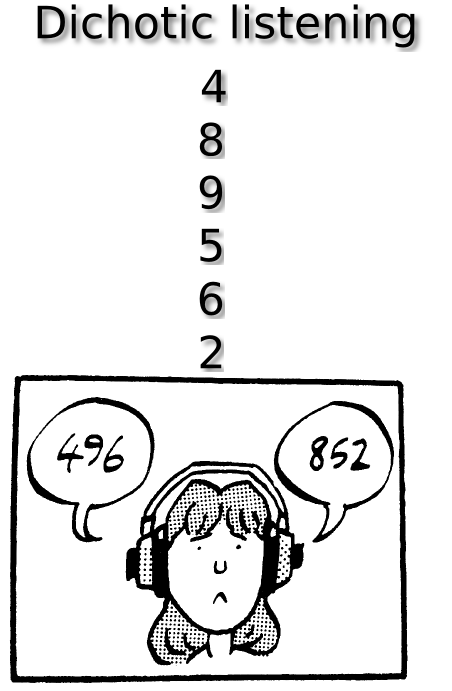
\includegraphics[width=35mm]{figs/l1/dichotic_listening_task.png}
 \end{center} 
\end{frame}


\begin{frame}
 \frametitle{Overview}
\begin{itemize}[<+->]
  \setlength{\itemsep}{5pt}
 \item Experimental paradigms for studying attention
 \begin{itemize}
  \item in space
  \item in time
 \end{itemize}
 \item Physiological basis of attention
 \item Disorders of attention
 \item Scene perception
\end{itemize}
\end{frame}

\begin{frame}
\frametitle{Attention}
\begin{overlayarea}{110mm}{80mm}
\begin{itemize}
 \item<1-> not a single \textit{thing} and does not have a single locus in the brain
 \item[]
 \item<2-> external vs. internal
 \item<3-> overt vs. covert
 \item<4-> focussed vs. divided
 \item<5-> sustained
 \item<6-> selective
\end{itemize}
\end{overlayarea}
\end{frame}


\begin{frame}
 \frametitle{Selection in space}
\begin{overlayarea}{130mm}{75mm}
\only<1->{
\begin{itemize}
 \item[] What does it mean to ``pay attention``?
\end{itemize}
}
\only<2->{
\begin{center}
\textcolor{blue}{Cueing paradigm} \begin{scriptsize}(Posner, 1980) \end{scriptsize}

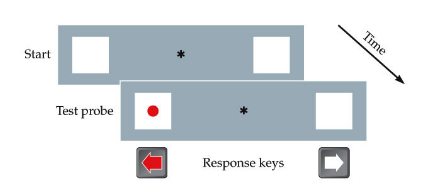
\includegraphics[width=80mm]{figs/l8/cueing_basic.png}
\end{center}
}

\only<3->{
Hit a response key as fast as possible when the probe appears!\\
\textbf{Dependent variable:} reaction time (RT)
}
\end{overlayarea}
\end{frame}



\begin{frame}
 \frametitle{Selection in space}
\begin{overlayarea}{110mm}{75mm}

\begin{center}
\textcolor{blue}{Cueing paradigm} \begin{scriptsize}(Posner, 1980) \end{scriptsize}
\end{center}
\begin{columns}[T]
 \begin{column}{50mm}
\centering valid
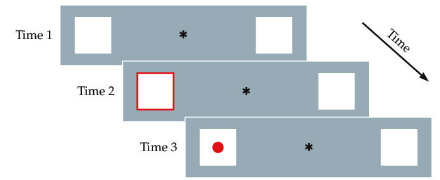
\includegraphics[width=60mm]{figs/l8/cueing_valid.png}
 \end{column}

 \begin{column}{80mm}
\centering invalid
 
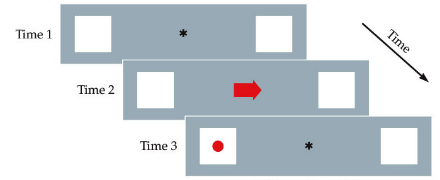
\includegraphics[width=60mm]{figs/l8/cueing_invalid.png}
 \end{column}
\end{columns}

\vspace{5mm}
\begin{itemize}
 \item<2->[Cue] stimulus that indicates where (or what) subsequent stimulus might be. Valid (giving correct information), invalid or neutral.
 \item<3-> exogeneous/peripheral vs. endogeneous/symbolic cues
 \item<4->[SOA] stimulus onset asynchrony  - time between onset of one stimulus and onset of another.
\end{itemize}
\end{overlayarea}
\end{frame}


\begin{frame}
\frametitle{Selection in scace}
\begin{overlayarea}{110mm}{75mm}
\begin{center}
\textcolor{blue}{Cueing paradigm} \begin{scriptsize}(Posner, 1980) \end{scriptsize}
\end{center}

 \begin{center}
\includegraphics<1-2>[width=70mm]{figs/l8/cueing_results.png}
 \end{center}
\begin{itemize}
 \item benefit from valid cue: $RT_{invalid} - RT_{valid}$
 \item increases with processing time for cue 
 \item peripheral cue is processed quicker
\end{itemize}
\end{overlayarea}
\end{frame}



\begin{frame}
\frametitle{Theories of Attention}
\begin{overlayarea}{110mm}{75mm}
\textbf{Spotlight model:}

\begin{itemize}
 \setlength{\itemsep}{5pt}
 \item attention is restricted in space and moves from one point to the next
 \item in-depth processing of areas within spotlight
\end{itemize}

\textbf{Zoom lens model:}

\begin{itemize}
 \setlength{\itemsep}{5pt}
 \item attended region can grow or shrink depending on the size of the area to be processed in detail
\end{itemize}
\end{overlayarea}
\end{frame}


\begin{frame}
 \frametitle{Visual Search}
\begin{overlayarea}{120mm}{70mm}
closer approximation of deployment of attention in the real world
\vspace{4mm}
\begin{columns}[T]
 \begin{column}{50mm}
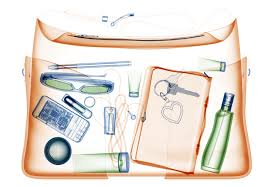
\includegraphics[width=40mm]{figs/l8/suitcase_scan.jpg}
 \end{column}

 \begin{column}{60mm} 
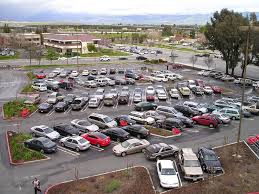
\includegraphics[width=40mm]{figs/l8/car_in_parking_lot.jpg}
 \end{column}
\end{columns}

\vspace{4mm}
Find the \textit{target} item among \textit{distractor} items!
\begin{itemize}
 \item[] 
 \item<2->[] \textbf{target} - goal of visual search
 \item<2->[] \textbf{distractor} - any stimulus other than the target (in visual search)
 \item<2->[] \textbf{set size} - number of items in visual search display
\end{itemize}
\end{overlayarea}
\end{frame}

\begin{frame}
 \frametitle{Visual search}
\includegraphics<1>[width=110mm]{figs/l8/types_visual_search_displays.png}
\includegraphics<2>[width=110mm]{figs/l8/types_visual_search.png}
\end{frame}

\begin{frame}
 \frametitle{Visual Search}
\begin{center}
\includegraphics<1>[width=100mm]{figs/l8/types_visual_search_summary.png}
\end{center}

Efficiency is quantified as average RT as a function of set size 
\begin{itemize}
  \item search slope, $\frac{ms}{item}$
  \item the larger the slope the less efficient the search
 \end{itemize}

\end{frame}



\begin{frame}
\begin{block}{Activity}
Quantify your visual search performance in the activity on the following webpage \url{http://sites.sinauer.com/wolfe4e/wa07.02.html}
 \end{block}
\end{frame}


\begin{frame}
 \frametitle{Using search efficiency to explore visual processing}
\begin{overlayarea}{110mm}{70mm}
\begin{columns}[T]
\begin{column}{40mm}
\includegraphics<1>[width=40mm]{figs/l8/feature_search.png}
\includegraphics<2>[width=40mm]{figs/l8/enns_rensink.png}
\end{column}

\begin{column}{70mm}
\begin{itemize}
 \item \textbf{feature search} - target defined by presence of single feature
 \item ''pop out`` of the target because of its saliency
 \item color or orientation can be processed at once - parallel search 
 \item[]
 \item<2-> look for the odd one out
 \item<2-> overall shape and orientation same, 
 \item<2-> difference in perceived depth \textbf{feature difference}
\end{itemize}
\end{column}
 \end{columns}
\end{overlayarea}
\end{frame}


\begin{frame}
 \frametitle{Using search efficiency to explore visual processing}
\begin{overlayarea}{110mm}{70mm}
\begin{columns}[T]
\begin{column}{40mm}
\includegraphics<1>[width=40mm]{figs/l8/serial_search.png}
\includegraphics<2>[width=40mm]{figs/l8/chinese_search.png}
\end{column}

\begin{column}{70mm}
\begin{itemize}
 \item \textbf{conjunction search} - target defined by co-occurrence of more than one feature
 \item each additional distractor adds a fixed amount of search time
 \item slope in trials without target twice as large as slope in trials with target 
 \item[$\rightarrow$] serial self-terminating search
 \item[]
 \item<2-> hardest search except you read Chinese
 \item<2-> T-among-L is simpler ''target hides in plain sight''
\end{itemize}
\end{column}
 \end{columns}
\end{overlayarea}
\end{frame}

\begin{frame}
 \frametitle{Real-world searches}
\begin{center}
\includegraphics<1>[width=80mm]{figs/l8/real_world_search.png}
\end{center}
In real-life search is often \textbf{guided:} Attention is restricted to a subset of possible items on the basis of information about the target's basic features (e.g., its color)
\end{frame}

\begin{frame}
 \frametitle{Attending in time}
\end{frame}


\begin{frame}
 \frametitle{References}
\begin{small}
\begin{itemize}
 \item  Wolfe, J.M., Kluender, K.R. \& Levi, D.M. (2012).\textit{Sensation \& Perception}. Sinauer Associates: Sunderland, MA. 
\end{itemize}
\end{small}
\end{frame}


\end{document}